\documentclass[11pt]{article}
\usepackage[margin=1.2in]{geometry}
% \usepackage{showframe}
\usepackage{caption}
\usepackage{float}
\usepackage{enumerate}
\usepackage{array}
\usepackage{graphicx}
\usepackage{setspace}
\usepackage{hyperref}
\setstretch{1.2}

\author{Nicole Loncke \& Lucianne Walkowicz}
\date{June 29, 2014}
\title{Efficiently Searching for Stellar Flares in Kepler Mission Data}

\begin{document}

\maketitle{}

% Section 1:
% A few corrections: Kepler stares at one one part of the sky, and does
% so for *years* at a time, broken into 3 month chunks. You can refresh
% your Kepler knowledge at kepler.nasa.gov (and you should probably
% include a footnote with that URL as a reference). 
\section{Introduction}
\label{sec:intro}
The Kepler Mission is designed to survey our galaxy in the hopes of
discovering planets in or near the habitable zone of their stars.  In
doing so, it will become possible to determine how many of the
billions of stars in our galaxy have such planets. Kepler's 0.95-meter
diameter telescope has been staring at one portion of the sky for 5+
years to gather brightness data about these stars\footnote{For more
  information, see http://kepler.nasa.gov/ and
  http://www.nasa.gov/mission\_pages/kepler/overview/index.html}.  In
addition to planet detection, this data can be used to gather
properties about the $10^5$ stars within the field.  In this paper we
are concerned with the flaring behaviors of these nearby stars and
discovering techniques we can use to better determine their effect on
the environments of any orbiting planets.

\section{The Data and Motivation}
\label{sec:data}
The data we chose to investigate are from Quarter 9 of Kepler's
collection.  This corresponds to the 3-month period from mid-March to
late June 2011.  Within that time window, we examined M dwarf stars in
particular.  M dwarfs comprise about 75\% of the stars in our galaxy
so they are primary candidates for investigation, if only due to their
widespread representation in our neighborhood and in the universe.
Furthermore, M dwarfs are highly magnetically active---when magnetic
field lines snap and reconnect, the resulting outpourings of energy
can have drastic effects on the conditions of nearby
planets.\footnote{Hilton et al., ``The Galactic M Dwarf Flare Rate,''
  2010.}

Our over-arching goal was to collect measurements on the frequency and
intensity of flares for each light curve.  The process is two-fold:
first, one must correctly identify the flares in the data; secondly,
one must compute the frequencies and intensities, then analyze the
results.  In the following section, we discuss the code we wrote to
assist in performing these tasks.

% We found that the existing methods for the first step were highly
% inefficient and spend much of the paper discussing and evaluating
% our ideas for improvement

\section{Our Tools}
\label{sec:tools}
One rudimentary method of finding the flares is to flag those points
in the light curve that have brightness above a certain threshold.  We
have written a program in IDL that does this and must verify by-eye
all of the events it flags as flares.  
% For stronger motivation have some statistic on how well the IDL
% program does---what percentage of the flagged events did you label
% as y's?
To do so, we have also written a Python module, \verb|lightcurves.py|,
to aid in the vetting process.

\subsection{Formatting}
\label{sec:format}
The \verb|lightcurves| module makes some assumptions about the format
of the input data.  The light curve data should be in a file
containing a whitespace-separated table with time in the first column
and flux in the second.
\begin{table}[h]
  \centering
  \begin{tabular}{>{\itshape}p{0.2\linewidth} >{\itshape}l}
       808.51470   &   6338.22 \\
       808.53514   &   6340.73 \\
       808.55557   &   6346.89 \\
       808.57601   &   6341.10 \\
       808.59644   &   6340.22 \\
  \end{tabular}
  \caption{Light curve data sampled from Kepler ID 10068383.}
\end{table}

The other fundamental input file is the one containing the potential
flare events, or ``flags,'' generated by the IDL program.  This file
contains one column listing indices into the time array at the points
that mark a suspected event.  The module functions use the light curve
data and flags thusly formatted as inputs for vetting.

% Section 2.2: I'm seeing what you mean by tense changes here-- the ``if
% you X'' and ``if your aim is X'' stuff is what makes it still read
% like documentation! Try taking out sentences like this and replacing
% them with simple statements of what the function actually *does*, such
% as ``The ltcurve() function reads a single data file and displays it
% in a plot for inspection''. 

\subsection{Plotting}
\label{sec:basic}
The \verb|ltcurve()| function takes as its primary argument a string
of the name of the file containing the Kepler data and returns the
time and brightness arrays.  By default it also displays the light
curve corresponding to the file on a time vs. brightness plot, but
this feature can be switched off by passing the function an optional
argument.

The \verb|ltcurves()| function displays multiple light curve files one
at a time.  Its only required argument is a list or array of filename
strings. This function also accepts a keyword argument
\verb|flags|---a list of corresponding event flags for each of the
Kepler data files---with which it overplots the potential
flares.\footnote{These flags are generated using \texttt{getflags()}
  by passing it a list of the names of the files holding the flare
  flags.}

\subsection{Vetting}
\label{sec:vet}

Instead of cycling through the light curves with overplotted flags,
you may find it helpful to inspect and record whether or not the
marked events could potentially be stellar flares.  In that case, you
should use \verb|flareshow()|, which writes user input (either 'y',
'n', 'm') to two files for later retrieval.  See examples of the
display in figures \ref{fig:yes}, \ref{fig:no}, and \ref{fig:maybe}.
\begin{figure}[h!]
  \caption{A true stellar flare, displayed with flareshow().}
  \label{fig:yes}
  \centering
    \includegraphics[width=\textwidth]{plot_yes_zoom}
\end{figure}

\begin{figure}[h!]
  \caption{A falsely flagged event.}
  \label{fig:no}
  \centering
    \includegraphics[width=\textwidth]{plot_no_zoom}
\end{figure}

\begin{figure}[h!]
  \caption{An indeterminate event.}
  \label{fig:maybe}
  \centering
    \includegraphics[width=\textwidth]{plot_maybe_zoom}
\end{figure}

One file contains a space-separated table of the Kepler IDs and the
corresponding user responses to its events, see Table
\ref{tab:output}.  The other file contains information about the
length of each event, as displayed in Table \ref{tab:outputindices}.
These two files work in conjunction to gather more information about
the potential flares.
\begin{table}[h]
  \centering
  \begin{tabular}{l l}
    8848271 &  n \\
    8908102 &  n \\
    8953257 &  n  n  n  n  n  n  n  n \\
    9002237 &  n  n  n  y \\
  \end{tabular}
\caption{Example output.txt file.}
\label{tab:output}
\end{table}

\begin{table}[!h]
  \centering
  \begin{tabular}{l l}

8848271 &  3735 03 \\
8908102 &  1757 03 \\
8953257 &  1454  6 1610  7 1890  4 2359  3 2516  4 2829  5 2985  6
3265  5 \\
9002237 &  3337  4 3547  5 3756  3 3967  4 \\
\end{tabular}
\caption{Corresponding example output\_indices.txt file.}
\label{tab:outputindices}
\end{table}

Note that before using \verb|flareshow()|, you must have your flags in
the proper format, generated by \verb|getflags()|.  This helper
function outputs a nested list of event indices given a list of the
names of the files containing the flags.

\section{Initial Approach}
\label{sec:initial}
In order to gather data about the flares, it is necessary to first
correctly identify the stellar flares within the Kepler data.  These
events have a very distinct shape and thus can be picked out in the
light curve data by a simple program with rudimentary accuracy.  We
have written such a program in IDL that takes note of points in the
light curve where the brightness exceeds a certain threshold.  Before
proceeding to collect data on the flares, we must first manually
verify all of the events it flags as flares.

To make this verification process easier, we have also written a
Python module, \verb|lightcurves.py|.  It contains functions that
display the light curves with the flagged points marked, in addition
to accepting and recording user input about whether the flags are
truly flare events.  We employed a combination of these tools to
inspect 212 light curves.  Out of the 315 events in that dataset that
were marked as potential flares using thresholding, we conclusively
determined 126 of them are flares.  Of the remaining events, 117 are
definitely not flares and the balance are indeterminate.



\section{Machine Learning}
\label{sec:ml}

This method of visually checking each event is slow, however, and the
major bottleneck for data analysis. Because the IDL flare detection
program that produces the flare flags does not correctly identify
events with high accuracy, much human effort is devoted to verifying
its output.  The thresholding performed by the program is only one
aspect of the process our human brains go through when inspecting
these light curves.  (See examples in Figures \ref{fig:yes},
\ref{fig:no}, and \ref{fig:maybe}.)  When we vet the flare events by
eye, the brain is actually comparing each event to a set of ideas---a
model---of what a real flare should look like in the data.

If we could write another program to build such a model from
quantitative metrics then we could train it to recognize the same
patterns that humans so easily detect in the light curves, thereby
nearly automating our task---obtaining stellar flare data from the raw
light curves with high confidence.  To accomplish this goal, we
trained a variety of machine classifiers on metrics from each
potential flare event and their respective light curves.


\subsection{Training}
\label{sec:train}
Our first task was to gather quantitative measurements of features for
each stellar flare to feed into the classifier.  In total we use 10
features.
\begin{enumerate}[(1)]
\item \emph{amplitude}: the range of the entire light curve.  Stars
  with great stellar variability tend to be more magnetically active
  than those without.  We expect high light curve amplitude to
  correlate with real flares.
\item \emph{number of events}: Light curves that have many flagged
  events tend to have real flares, so we expect a high number of
  events to correlate with real flares.
\item \emph{standard deviation}: The standard deviation of the entire
  light curve with stellar variability subtracted.  It may be useful
  to feed the classifier more information about the light curve at
  large.
\item \emph{consecutive points}: Sometimes there are gaps in the
  Kepler data.  Kepler must rotate and point its antenna towards Earth
  to send its light curve data roughly every month.  When the
  satellite begins recording again, there may be a sudden increase in
  brightness that resembles a flare but isn't.  In order to avoid
  marking these as true flares we check whether the time intervals are
  evenly spaced across the event.
\item \emph{kurtosis}: The kurtosis measures the ``peakedness'' of a
  flare event.  A sharp increase and decrease in brightness is likely
  to indicate a true flare, though the decay ought to be more gradual
  than the incline.
\item \emph{midpoint check}: A stellar flare typically requires a
  monotonic increase then monotonic decrease in brightness.  Ensuring
  that the middle point is higher than the beginning and end points of
  the event is one way to rule out falsely marked events.
\item \emph{second derivative}: Smoothing over the flagged event, is
  the light curve locally concave up or down?  The second derivative
  of the window around the potential flare can capture the shape of a
  light curve in the neighborhood of an event.
\item \emph{skew}: Skewness is a measure of the asymmetry of the event
  brightness---is the flare left-leaning or right-leaning?  Because
  flares are characterized by very quick increases in brightness
  followed by a slow decay, left-leaning events (and therefore those
  with negative skew) are more likely to be true flares.
\item \emph{slope}: Is the brightness of the star generally increasing
  or decreasing at the time of the event?  This metric measures the
  slope of the line formed by connecting the point at the beginning of
  the flare window to the point at the end of the flare window.
  time of the event?
\item \emph{slope ratio}: We also compute the ratio of the light
  curve's slope just before the event begins and the slope just after
  it ends.  We hope to capture more information about the local shape
  of the light curve with this metric.
\end{enumerate}
These data were gathered for 315 potential flaring events that we had
previously labelled by-eye.  Using these samples we originally formed
a training set of 150 events and a test set of 165 events.

\subsection{Classification Performance}
\label{sec:class}
We use Python's \verb|scikit-learn| package for our machine learning
framework\footnote{Scikit-learn: Machine Learning in Python, Pedregosa
  et al., JMLR 12, pp. 2825-2830, 2011.}.  The package is fully
equipped with a suite of regression, clustering,
dimensionality-reduction, and classification tools.  Of the methods
available, we chose to experiment with support vector machines,
decision trees, and linear discriminant analysis.  Our target classes
are `y' for definitely a flare, `n' for not a flare, and `m' for any
indeterminate events.

To quantitatively compare the classifiers, it is important that we
define a few statistics related to their performance.  We say the
\emph{precision}, or \emph{efficiency}, is the fraction of events
classified as a given type (`y', `n', `m') that are truly of that
type.  The \emph{recall}, or \emph{completeness} of the classifier is
the fraction of objects that are truly of a given type that it
classifies as that type.  The $F_1$\emph{-score} is a weighted average of
recall and precision.

Though we ideally seek high scores for both precision and recall, for
our purposes precision is the more important metric.  Because we have
many events in our Kepler dataset it is better to correctly identify a
small number of flares and miss a few than to find many more true
flares at the expense of false positives.


\subsubsection{Support Vector Classification}
\label{sec:svc}
For our first attempt we used support vector classification as
packaged in \verb|sklearn.svm.SVC|. We initially used a linear kernel
SVM. This is a simple classification method which assumes that there
is a hyperplane that separates the data in the feature space, which is
10-dimensional in our case.  We trained our linear SVC on 150 flare
events and then used it to predict the status of 165 events.  This
classifier had a precision of 63\% for classifying true flare events.
While the results were better than a coin toss, we sought to improve
the classifier performance.

Sometimes the data cannot be linearly separated within the given
feature-space.  Alternate SVM kernels implicitly map the data to
higher dimensions to find a separating hyperplane.  To do that, we
incorporated the popular radial basis function (RBF) kernel into our
support vector machine model.  While support vector classification
with an RBF kernel does decently when predicting the flares it has
already seen, it does not outperform when predicting unseen events,
which is ultimately what is important. The results are charted in
tables \ref{tab:rbftrain} and \ref{tab:rbftest}.

\begin{table}
  \centering
  \begin{tabular}[!htbp]{c|c c c c}
        & precision &recall &$F_1$-score &support \\ \hline
    n   & 0.62      &0.87   &0.72     &60      \\
    y   & 0.63      &0.69   &0.66     &65      \\
    m   & 0.50      &0.12   &0.20     &40      \\ \hline
    avg & 0.60      &0.62   &0.57     &165     \\
  \end{tabular}
  \caption{Linear kernel performance with the test set.}
  \label{tab:lintest}
\end{table}

\begin{table}
  \centering
  \begin{tabular}[!htbp]{c|c c c c}
        & precision &recall &$F_1$-score &support \\ \hline
    n   & 0.73      &0.81   &0.77     &57      \\
    y   & 0.74      &0.89   &0.81     &61      \\
    m   & 0.71      &0.31   &0.43     &32      \\ \hline
    avg & 0.73      &0.73   &0.71     &150     \\
  \end{tabular}
  \caption{Reconstructing the training set with RBF kernel.}
  \label{tab:rbftrain}

  \begin{tabular}[!htbp]{c|c c c c}
        & precision &recall &$F_1$-score &support \\ \hline
    n   & 0.61      &0.88   &0.72     &60      \\
    y   & 0.62      &0.60   &0.61     &65      \\
    m   & 0.33      &0.12   &0.18     &40      \\ \hline
    avg & 0.55      &0.59   &0.55     &165     \\
  \end{tabular}
  \caption{RBF kernel performance on the testing set.}
  \label{tab:rbftest}
\end{table}


\subsubsection{Random Forest Classifier}
\label{sec:randfor}
We performed the same task using random forest classification, as
packaged in \verb|sklearn.ensemble|.  The algorithm constructs many
decision trees based on the inputs it sees during the training phase,
then uses those trees to predict the categories of unseen
samples. While it performed superbly on the training set, it performed
no better than our support vector machines on the test set.

\begin{table}
  \centering
  \begin{tabular}[!htbp]{c|c c c c}
       & precision &recall &$F_1$-score &support \\ \hline
    n  & 1.00      &0.92   &0.99     &57      \\
    y  & 0.95      &1.00   &0.98     &61      \\
    m  & 1.00      &0.94   &0.97     &32      \\ \hline
    avg& 0.98      &0.98   &0.98     &150     \\
  \end{tabular}
  \caption{Reconstructing the training set with random forest classification method.}

  \begin{tabular}[!htbp]{c|c c c c}
       & precision &recall &$F_1$-score &support \\ \hline
    n  & 0.63      &0.77   &0.69     &60      \\
    y  & 0.60      &0.72   &0.66     &65      \\
    m  & 0.29      &0.10   &0.15     &40      \\ \hline
    avg& 0.54      &0.59   &0.55     &165     \\
  \end{tabular}
  \caption{Random forest method performance on the testing set.}
\end{table}

\subsubsection{Linear Discriminant Analysis}
\label{sec:lda}
Lastly, we used the linear discriminant analysis method (LDA), which
attempts to model the difference between the classes as linear
combinations of the features
\footnote{\url{http://www.ics.uci.edu/~welling/classnotes/papers_class/Fisher-LDA.pdf}}.
LDA is closely related to principal component analysis in that it also
performs dimensionality reduction, but it uses the given class labels
to function as a linear classifier. (PCA is an unsupervised technique;
it does not perform classification.)
\begin{table}
  \centering
  \begin{tabular}[!htbp]{c|c c c c}
       & precision &recall &$F_1$-score &support \\ \hline
    n  & 0.72      &0.86   &0.78     &57      \\
    y  & 0.70      &0.84   &0.76     &61      \\
    m  & 0.67      &0.19   &0.29     &32      \\ \hline
    avg& 0.70      &0.71   &0.67     &150     \\
  \end{tabular}
  \caption{Reconstructing the training set with LDA.}

  \begin{tabular}[!htbp]{c|c c c c}
        & precision &recall &$F_1$-score &support \\ \hline
    n   & 0.63      &0.83   &0.72     &57      \\
    y   & 0.60      &0.71   &0.65     &61      \\
    m   & 0.56      &0.12   &0.20     &32      \\ \hline
    avg & 0.60      &0.61   &0.57     &150     \\
  \end{tabular}
  \caption{LDA performance on the testing set.}
\end{table}
Our LDA classifier performed with 60\% precision and 71\% completeness
for the true flares, which is comparable to the other three methods.

% Conclusions: You should note here that while the human element hasn't
% been completely removed, the amount of human intervention required is
% MUCH, much less using this method than it would be. Remember that
% you've only had to look at 300ish flares-- but there are roughly
% 30,000 stars we can apply this to for every 3 month chunk of Kepler
% data over the past five years. That would be impossible to do if
% humans had to do all the vetting by eye!

\section{Conclusion}
\label{sec:conc}
We set out to gather data about flaring stars in order to explore the
impact that these stars might have on the conditions of nearby
planets.  Processing the light curves to identify flares, however,
required a large human component in the form of looking at each curve
and manually recording the status of each event.  Our dataset
consisted of light curves for only 212 stars but there are roughly
30,000 stars we can analyze for every 3 month chunk of Kepler data
over the past five years---by-eye vetting is an impractical method in
the long term.

In an effort to automate flare detection, we employed machine learning
techniques to classify a set of pre-vetted events.  Of the four
classifiers used---SVM with linear kernel, SVM with radial basis
function kernel, random forest, and linear discriminant
analysis---performance metrics suggest that the simple linear support
vector machine is the best choice for our task, as it has the best
precision score for the test data.

There is still much room for performance improvement, however.  As
with many classification problems, increasing the size of the training
set can significantly improve prediction accuracy.  Doing so requires
more labelled data which means we must, ironically, vet more potential
flares by eye.  As a diagnostic for expected improvement we have
plotted a learning curve (accuracy as a function of training set size)
for each of the different classifiers.  See Figures \ref{fig:lc_lin},
\ref{fig:lc_rf}, and \ref{fig:lc_lda}. These plots show that the
classifiers have simply not seen enough variety in the training set to
be able to classify new inputs.  There are no signs of convergence to
a low error rate.  Had the learning curves already plateaued with a
training set of 150 samples then providing more samples would not
significantly improve prediction accuracy.

\begin{figure}[h!]
  \caption{Learning curve for linear kernel support vector machine.}
  \label{fig:lc_lin}
  \centering
    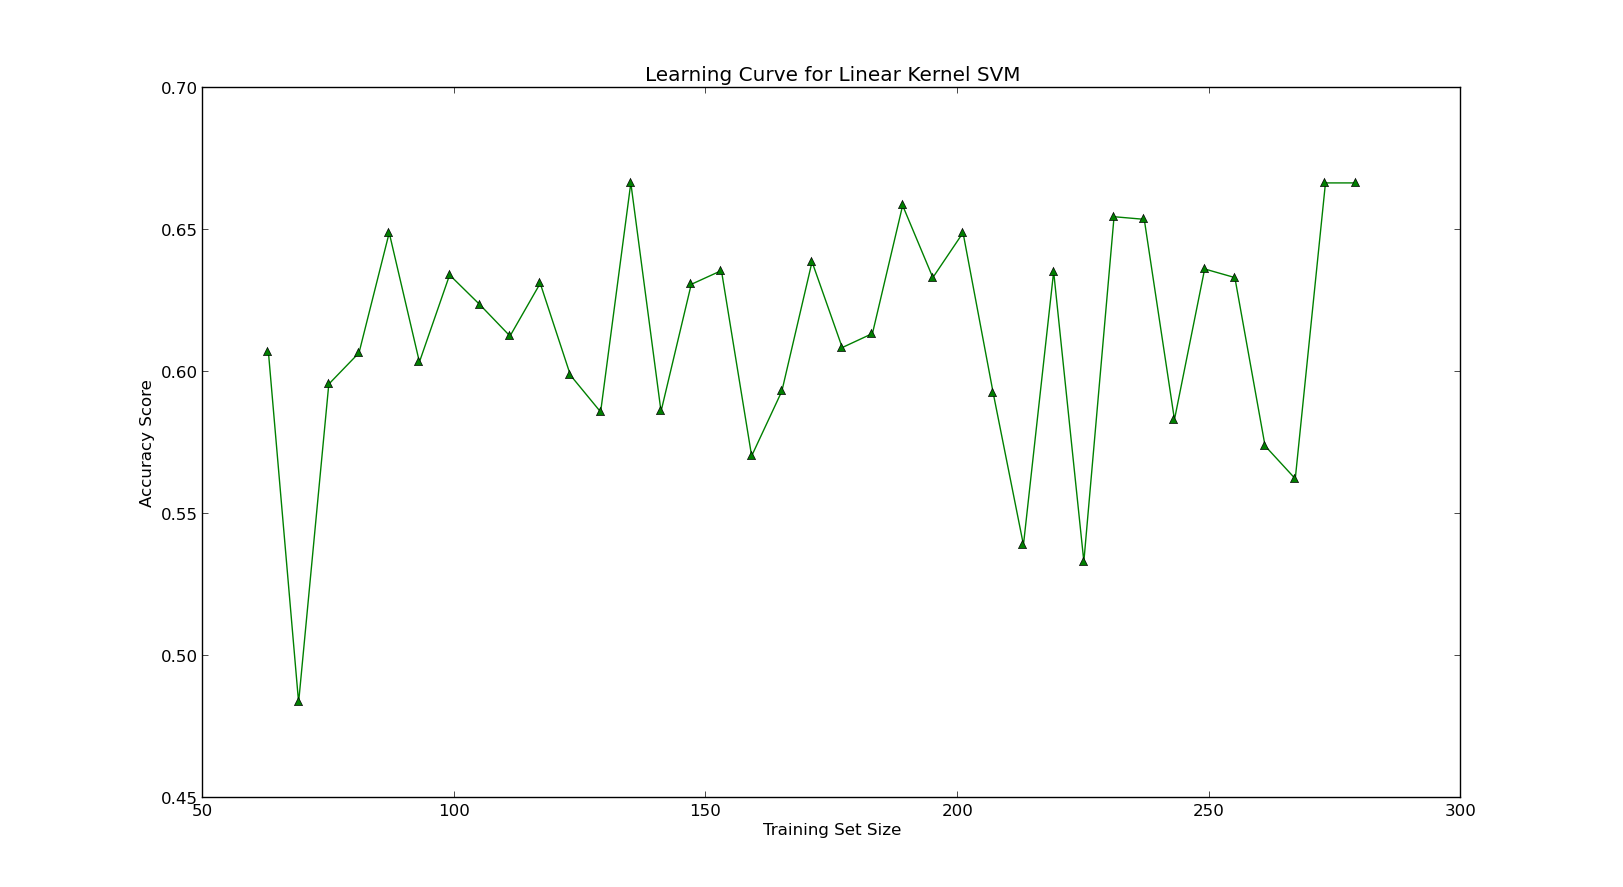
\includegraphics[width=\textwidth]{learncurve_linear}
\end{figure}

\begin{figure}[h!]
  \caption{Learning curve for random forest classifier.}
  \label{fig:lc_rf}
  \centering
    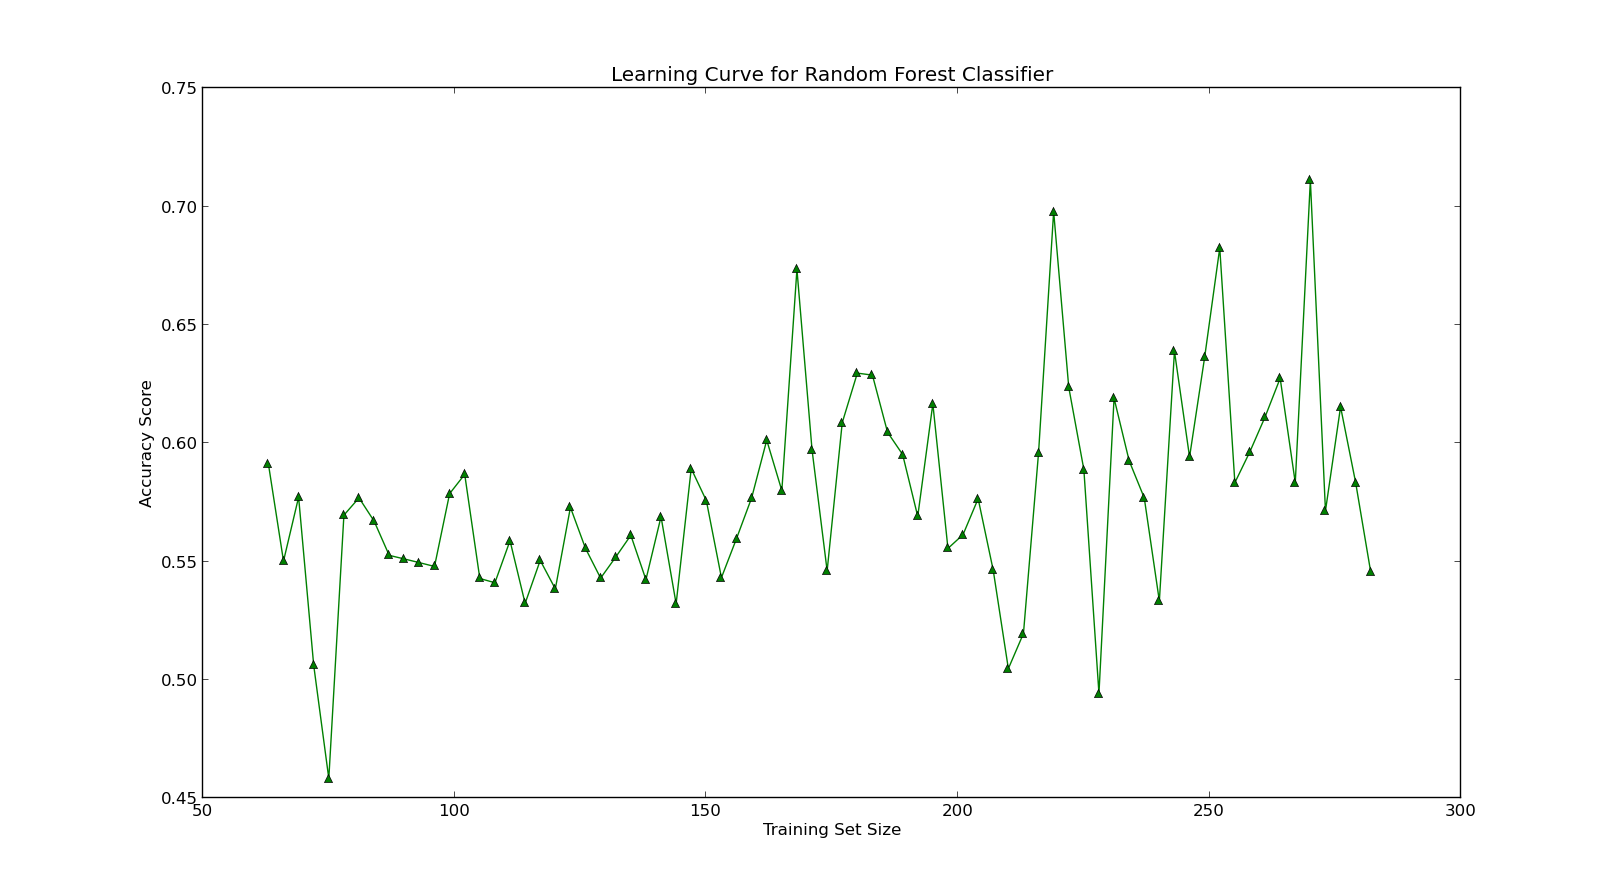
\includegraphics[width=\textwidth]{learncurve_randfor}
\end{figure}

\begin{figure}[h!]
  \caption{Learning curve for linear discriminant analysis.}
  \label{fig:lc_lda}
  \centering
    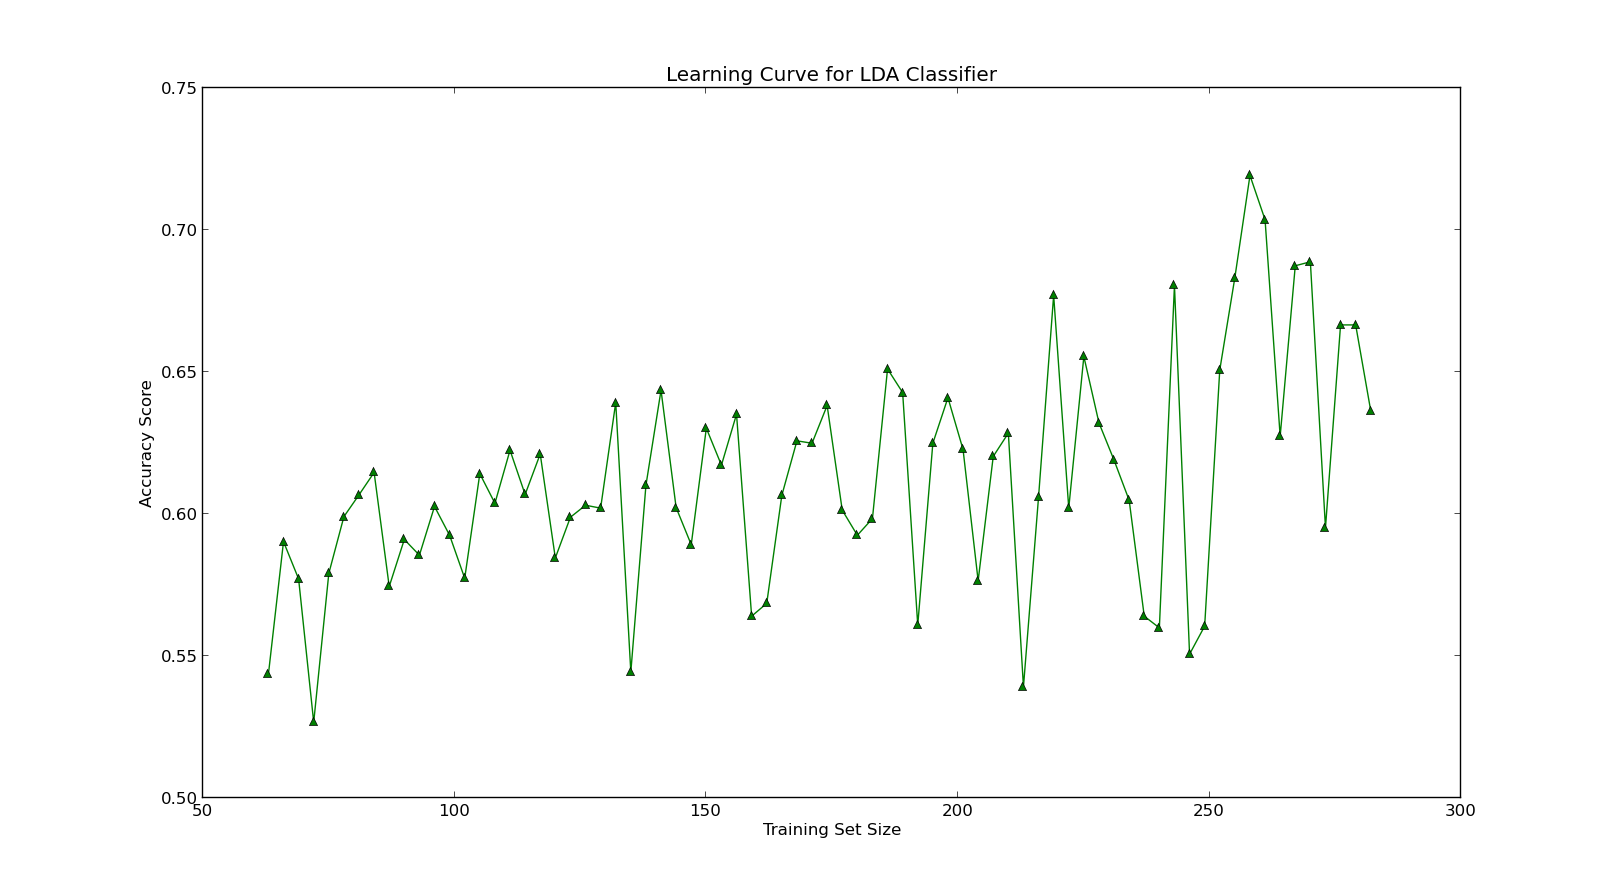
\includegraphics[width=\textwidth]{learncurve_lda}
\end{figure}

The advantage of being able to test the classifiers on labelled data
is that we can see how many of the flares are being incorrectly
identified.  With this knowledge, there may be a way to correct for
those flares that are misjudged by our algorithms.  Pre-processing the
data (e.g. scaling the features to be within a similar range) and
additional data science techniques may help improve our classifiers'
accuracy\footnote{We plan on investigating some of the measures
  discussed here:
  \url{http://www.csie.ntu.edu.tw/~cjlin/papers/guide/guide.pdf}}.

Currently, we have yet to completely remove the human element from
detecting light curves, but with the the machine learning techniques
mentioned we have much higher hopes for doing so.
\end{document}